\chapter{Processi e threads}
Il concetto centrale per ogni sistema operativo \'e quello di processo, l'astrazione di un programma che sta venendo eseguito. Tali astrazioni permettono
di avere operazioni pseudo-concorrenti anche quando esiste una sola CPU, trasformandola in diverse CPU virtuali.
\section{Processi}
Tutti i computer moderni svolgono diverse funzioni allo stesso tempo. In un sistema multiprogramma la CPU cambia da processo a processo rapidamente,
eseguendo ognuno per decine o centinaia di millisecondi. Si parla di pseudoparallelismo in contrasto con il parallelismo dei sistemi multiprocessore. .
\subsection{Il modello dei processi}
In questo modello tutti il software eseguibile sul computer \`e organizzato in un numero di processi sequenziali, istanze di un programma che sta venendo eseguito con i valori per
il contatore, i registri e le variabili. Ogni processo possiede la propria CPU virtuale, anche se \`e la CPU che cambia tra i processi, chiamato multiprogramming. Ogni programma in
questo caso viene eseguito in maniera indipendente. Essendo che esiste un unico contatore di programma fisico, quando un processo viene eseguito il suo contatore logico \`e inserito
in quello reale. Quando si passa ad un altro processo il contatore fisico \`e salvato nel contatore logico del processo. Si assuma che ci sia una sola CPU. Con essa che cambia tra i
processi, il tasso di computazione di un processo non sar\`a uniforme n\`e riproducibile, pertanto i processi non possono essere programmati con assunzioni riguardo alla temporizzaizone.
Quando un processo richiede dei criteri real-time eventi si devono prendere delle misure speciali. Il processo pu\`o essere considerato come un'istanza del programma, con un input, un
output e uno stato. Si noti come se un programma viene eseguito due volte conta come due proessi.
\subsection{Creazione dei processi}
I sistemi operativi necessitano di un modo per creare processi. In sistemi progettati per eseguire una singola applicazione potrebbe essere possibile avere tutti i processi che saranno
necessari presenti allo startup. In sistemi general-purpose \`e neccessario avere qualche modo per creare e terminare processi quando sono necessari durante l'operazione. Ci sono
quattro princupali cause per la creazione di un processo:
\begin{itemize}
	\item Inizializzazione del sistema. Durante la fase di boot sono creati numerosi processi, alcuni che interagiscono con l'utente e altri di background che non sono associati con
	      utenti particolari ma hanno funzioni specifiche. I processi che stanno nel background per gestire delle attivit\`a sono detti daemons e sistemi grossi ne possiedono a
	      dozzine.
	\item Esecuzione di una system call da un processo che sta venendo eseguito che crea un processo attraverso una system call. Creare un nuovo processo \`e utile quando il lavoro
	      che deve essere eseguito pu\`o essere formulato come un insieme di processi che interagiscono ma sono indipendenti.
	\item L'utente richiede di creare il processo in sistemi interattivi attraverso un comando o cliccando su un'icona. In sistemi basati su UNIX il nuovo processo rileva la finestra
	      da dove \`e eseguito. In windows il processo pu\`o creare una o pi\`u finestre. In entrambi i casi l'utente pu\`o avere pi\`u finestre aperte contempoaneamente.
	\item Inizializzazione di un batch job su sistemi batch che si trovano su grandi mainframes. Gli utenti possono inviare batch jobs al sistema e quando il sistema decide che ha
	      le risorse necessarie per eseguirne un altro crea un nuovo processo e svolge il job successivo nella coda.
\end{itemize}
Tecnicamente in tutti questi casi un nuovo processo \`e creato avendo un processo esistente che esegue una system call che dice al sistema operativo di creare un nuovo processo e indica
direttamente o indirettamente quale programma eseguire in esso. In UNIX esiste un'unica system call per creare un nuovo processo: \emph{fork} che crea un clone esatto del processo
chiamante. Dopo la \emph{fork} i due processi hanno la stessa immagine di memoria, le stesse stringhe ambientali e gli stessi file aperti. Tipicamente il processo figlio esegue
\emph{execve} o una system call simile per cambiare l'immagine di memoria e eveguire un nuovo programma. Quando l'utente inserisce un comando la shell forka il processo figlio che poi
esegue il comando. QUesti due passaggi permettono al figlio di manipolare i propri file descriptors dopo la \emph{fork} ma prima dell'\emph{execve}. In Windows una singola chiamata alla
funzione \emph{CreateProcess} gestisce entrambi i passaggi con $10$ parametri che includono la creazione e il caricamento del programma corretto da eseguire, i parametri di liena di
comando, attributi di sicurezza, bit di controllo e un puntatore alla struttura in cui le informazioni sul processo sono ritornate al chiamante. Dopo che un processo \`e creato
il genitore e il figlio possiedono i propri spazi di indirizzamento distinti. In UNIX quello del figlio \`e inizialmente una copia del genitore ma non \`e condivisa memoria scrivibile.
\subsection{Terminazione di un processo}
Dopo che un processo \`e stato creato e ha svolto il suo lavoro termina in:
\begin{itemize}
	\item Normal exit (volontaria), la maggior parte dei processi termina in questo modo eseguendo una system call in modo da dire al sistema operativo che ha finito.
	      Questa call \`e \emph{exit} in UNIX e \emph{ExitProcess} in Windoes. Programmi screen-oriented supportano la terminazione volontaria.
	\item Error exit (volontaria), avviene quando il processo scopre un errore, lo annuncia ed esce, le applicazioni screen oriented tipicamente creano una dialog box.
	\item Fatal error (involontaria) \`e causata da un bug nel programma, come l'esecuzione di un'istruzione illegale.
	\item Ucciso da un altro processo (involontario) attraverso una system call che dice al sistema operativo di terminarlo in UNIX \`e \emph{kill}, in Windows \`e
	      \emph{TerminateProcess}.
\end{itemize}
In alcuni sistemi quando un processo termina sono uccisi anche tutti i processi che ha creato.
\subsection{Gerarchie di processi}
In alcuni sistemi quando un processo ne crea un altro rimangono associati in certi modi. in UNIX un progesso e tutti i suoi discendenti formano un gruppo di processi. Quando un segnale
viene inviato dalla tastiera viene ricevuto da tutti i membri del gruppo di processi associati alla tastiera. Individualmente ogni processo pu\`o catturare il segnale, ignorarlo o
svolgere un'azione default, che \`e di essere ucciso dal sengale. Un altro esempio di gerarchia \`e dato dal inizializzazione di UNIX successivamente la fase di boot. Un processo
speciale detto \emph{init} \`e presente nella immagine di boot e quando viene eseguito legge un file che dice quanti terminali ci sono. Successivamente forka ad un nuovo processo per
terminale. Questi processi aspettano per un login che se hanno successo esegue una shell per eseguire comandi che potrebbero iniziarne altri e cos\`i via. Pertanto tutti i processi
del sistema si basano su un singolo albero con \emph{init} alla radice. Windows non possiede un concetto di gerarchia dei processi: sono tutti uguali, ma quando un processo \`e generato
il padre possiede un token detto handle che gli permette di controllare il figlio. Questo tolen pu\`o essere passato ad altri process, annullando la gerarchia.
\subsection{Stati dei processi}
Nonostante ogni processo sia un'entit\`a indipendente, con il proprio program counter e stato interno, deve spesso interagire con altri processi, ad esempio accettando come input
l'output di altri. Quando un processo si blocca lo sa in quanto non pu\`o continuare logicamente, tipicamente quando sta aspettando per un input che non \`e disponibile. \`E inoltre
possibile che sia bloccato in quanto il sistema operativo ha deciso di allocare la CPU per un altro processo. Queste due condizioni sono diverse in quanto la prima \`e inerente il
problema, mentre nel secondo caso \`e una tecnicalit\`a del sistema. Ci sono pertanto tre stati che il processo pu\`o avere:
\begin{itemize}
	\item Running: il processo sta utilizzando la CPU.
	\item Ready: eseguibile, stoppato per far eseguire un altro processo. Stato logicamente simile al primo in quanto il processo in entrambi i casi \`e capace di essere eseguito.
	\item Blocked: incapace di essere eseguito fino a che un evento esterno accade. Questo stato \`e differente in quanto il processo non pu\`o essere eseguito anche con la CPU
	      libera.
\end{itemize}
L'unica transizione non possibile \`e duella da ready a blocked. La transizione da running a blocked avviene quando il sistema scopre che un processo non pu\`o contineare al momento.
In alcuni sistemi si pu\`o eseguire una system call come \emph{pause} per entrare in uno stato bloccato, in altri sistemi come UNIX, quando un processo legge da una pipe o da un file
speciale e non si trova input disponibile il processo \`e automaticamente bloccato. La transizione da running a ready e viceversa sono causate dallo scheduler dei processi in modo da
permettere l'eventuale esecuzione di tutti i processi in stato ready. La transizione da blocked a running avviene quando un evento esterno elimina il blocco logico del processo.
Il modello dei processi permette di semplificare gli eventi interni al sistema: alcuni processi eseguono comandi dell'utente, altri sono parte del sistema e gestiscono richieste di
esso. Quando avviene un interrupt il sistema ferma il processo corrente ed esegue l'interrupt che si bloccano quando aspettano che accada qualcos altro. Il livello pi\`u basso del
sistema operativo \`e lo scheduler, con un insieme di programmi al di sopra di esso. Tutti i dettagli della gestione dell'interrupt e di blocco e inizio dei processi sono nascosti e il
resto del sistema operativo \`e stutturato in forma di processo.
\subsection{Implementazione dei processi}
Per implementare il modello dei processi il sistema operativo mantiene una tabella (array di strutture) chiamata la tabella dei processi con un entry per processo contenente
informazioni riguardo lo stato del processo, come il program counter, lo stack pointer, la memoria allocata, lo stato dei file aperti e le informazioni di accounting e scheduling e
ogni altra informazione che deve essere salvata quando il processo viene passato da running a ready o blocked in modo che possa essere fatto ripartire successivamente. In un tipico
sistema la tabella presenta tre colonne con la prima dedicata alla gestione del processo, la seconda alla gestione della memoria e la terza alla gestione dei file. Associato con ogni
classe di I/O si trova una locazione (tipicamente fissa al fondo della memoria) detta interrupt vector che contiene l'indirizzo dell procedura del servizio di interrupt. Quando accade
un interrupt tutti i processi che stanno venendo eseguiti salvano il program coutner, lo stato e dei registri nello stack grazie all'hardware di interrupt e il computer salta
all'indirizzo specificato nell'interrupt vector che fa partire la procedura. Tutti gli interrupt cominciano con il salvataggio dei registri nell'entri del processo corrente, dopo
l'informazione \`e pushata sullo stack dall'interrupt \`e rimossa e il puntatore allo stack \`e settato a puntare ad uno stack temporaneo utilizzato dal gestore dei processi. Il
salvataggio dei registri e il settaggio dello stack pointer devono essere svolti da una piccola routine in assembly, uguale per ogni interrupt. Quando la routine \`e finita chiama una
procedura in $C$ che svolge il resto del lavoro specifico al tipo di interrupt. Quando \`e finito viene chiamato lo scheduler per vedere quale processo deve essere eseguito. Dopo
quello il controllo \`e passato al codice in assembly per ricaricare in memoria i registri e le mappe per il proceso corrente e comincia ad essere eseguito. Dopo ogni interrupt il
processo ritorna precisamente nello stesso stato in cui era prima che accadesse l'interrupt. Riassumendo il processo di interrupt:
\begin{itemize}
	\item L'hardware salva lo stato del processo sullo stack.
	\item L'hardware carica il nuovo program counter dall'interrupt vector.
	\item Una procedura in assembly salva i registri.
	\item Una procedura crea un nuovo stack.
	\item Una servizio di interrupt in C viene eseguito (tipicamente legge e buffera l'input).
	\item Lo scheduler decide il prossimo processo da eseguire.
	\item Una procedura in C ritorna il codice in assmbly.
	\item Una procedura in assembly ricomincia il nuovo processo corrente.
\end{itemize}
\subsection{Modellare la multiprogrammazione}
L'utilizzo della multiprogrammazione permette il miglioramento dell'utilizzo della CPU: se il processo medio computa il $20\%$ del tempo che risiede in memoria, $5$ processi alla volta
dovrebbero rendere la CPU occupata tutti il tempo (irrealisticamente ottimistico). Un modello migliore consiste nel guardare l'utilizzo della CPU in modo probabilistico: suppondendo che
un processo utilizzi una frazione $p$ del suo tempo aspettando per il completamento dell'I/O. Con $n$ processi in memoria alla volta, la probabilit\`a che tutti gli $n$ processi stiano
aspettando per l'I/O \`e $p^n$, pertanto l'utilizzo della CPU \`e $1-p^n$. \`E facile notare come siano richiesti molti processi per rendere efficiente l'utilizzo della CPU. Si devono
naturalmente fare delle assunzioni: tutti i processi sono indipendenti mentre con una singola CPU non si possono avere processi che vengono svolti in contemporanea. Pur non essendo
preciso, questo modello d\`a una buona approssimazione delle prestazioni della CPU.
\section{Threads}
Nei sistemi operativi tradizionali ogni processo possiede uno spazio di indirizzamento e un singolo thread di controllo e nonostante questo \`e desiderabile avere multipli thread di
controllo nello stesso spazio di indirizzamento eseguiti quasi in parallelo, quasi come processi separati.
\subsection{Utilizzo dei thread}
La ragione principale alla base dell'utilizzo dei thread \`e che molte applicazioni possiedono multiple attivit\`a che avvengono insieme. Alcune di queste potrebbero bloccarsi. Una
decomposizione in multipli thread sequenziali semplifica il modello di programmazione. Si nota l'analogia con la neccessit\`a di avere i processi, con l'unica differenza che i thread
permettono a entit\`a parallele di condividere uno spazio di indirizzamento e tutti i dati tra di loro, un'abilit\`a fondamentale per certe applicazioni. Oltre a questo i thread sono
pi\`u leggeri e veloci da creare e distruggere dei processi, propriet\`a utile per un sistema dinamico e rapido. Permettono anche una certa sovrapposizione di attivit\`a non legate alla
CPU. Invine sono utili in sistemi con multiple CPU, dove il parallelismo \`e possibile. Esiste un modello di progetatzione in cui lo stato di computazione deve essere salvato e
ripristinato nella tabella ogni volta che si cambia tra le richieste, simulando i threads e i loro stack, chiamato macchine a stato-finito. I thread rendono pertanto possibile mantenere
l'idea dei processi sequenziali che fanno chiamate bloccanti e ottenere parallelismo:\\
\begin{tabular}{|c|c|}
	\hline
	\textbf{Modello}          & \textbf{Caratteristiche}                             \\
	\hline
	Threads                   & Parallelismo, system calls bloccanti                 \\
	\hline
	Processi a thread singolo & Assenza di parallelismo, system calls bloccanti      \\
	\hline
	Macchine a stato finito   & Parallelismo, system calls non bloccanti, interrupts \\
	\hline
\end{tabular}
\subsection{Il modello dei thread classico}
Il modello dei processi si basa sui concetti indipendenti di raggruppamento delle risorse ed esecuzione: i thread permettono la loro separazione. Si pu\`o considerare un processo come
un modo per raggruppare risorse imparentate insieme: possiede uno spazio di indirizzamento che contiene il programma e i dati e altre risorse come file aperti, processi figli, allarmi
in attesa, gestori di segnali, informazioni di gestione che uniti in esso sono gestiti pi\`u facilmente. Il processo inoltre possiede un thread di esecuzione che possiede un program
counter che traccia quale istruzione eseguire successivamente, registri che contengono le variabili correnti, uno stack con la storia dell'esecuzione con un frame per ogni procedura
senza ritorno. Pertanto se i processi raggruppano risorse i thread sono le entit\`a in programma per esecuzione sulla CPU. I thread permettono un esecuzione multipla sullo stesso
ambiente di processo con grande livello di indipendenza. Il termine multithreading \`e utilizzato per descrivere una situazione in cui sono presenti mutlipli thread, detti processi
leggeri. Quando un processo a muiltithread viene eseguito su un sistema a singola CPU i threads fanno a turno come i processi. Thread diversi in un processo non sono indipendenti come
processi diversi: possiedono lo stesso spazio di archiviazione e pertanto devono condividere le stesse variabili globali e possono accedere e modificare i rispettivi stack, non
necessaria in quanto i thread si generano da un processo generato da un utente e sono creati in modo da cooperare. Si nota come pertanto gli oggetti singoli di un processo sono lo
spazio di archiviazione, le variabili globali, file aperti, processi figli, allarmi in attesa, segnali e loro gestori e informazioni di contabilit\`a, mentre un thread possiede il
program counter, i registri, lo stack e lo stato. Nello stesso modo dei processi possono essere eseguiti, bloccati, pronti o terminati. Ogni stack del thread contiene un frame per
ogni procedura che \`e stata chiamata ma non ha ancora prodotto un valore di ritorno, distinta per ogni thread. Quando si trova multithreading i processi cominciano solitamente con un
unico thread presente che pu\`o crearne altri attraverso \emph{thread\_create} in cui un parametro specifica il nome della procedura per il nuovo thread. In alcuni casi possono essere
gerarchici. La creazione di un thread ritorna un identificatore del thread che lo nomina. Quando un thread ha finito esce chiamando \emph{thread\_exit} che lo fa svanire. In alcuni
sistemi pu\`o aspettare per l'uscita di un thread specifico attraverso \emph{thread\_join} che blocca il thread chiamante fino a che il thread specificato non ha finito. Un'altra
chiamata comune \`e \emph{thread\_yeld} che permette ad un thread di abbandonare la CPU per lasciare l'esecuzione per un altro thread. I thread generano delle complicazioni: la
creazione di un processo figlio genera problemi in quanto dovrebbe ereditare tutti i thread del padre in quanto potrebbero essere essenziale, ma cosa succede a questi ultimi se erano
bloccati da un interrupt. Un'altra classe di problemi dipende dal fatto che i thread condividono molte strutture dati che rendono necessaria una progettazione accurata.
\subsection{Thread POSIX}
Per rendere possibile la creazione di programmi con thread l'IEEE ha definito uno standard chiamato Pthreads supportato dalla maggior parte dei sistemi UNIX che definisce $60$ chiamate
a funzioni come:
\begin{itemize}
	\item \emph{Phtread\_create} che crea un nuovo thread.
	\item \emph{Phtread\_exit} che termina il thread chiamante.
	\item \emph{Phtread\_join} che aspetta per l'uscita di un thread specifico.
	\item \emph{Phtread\_yield} che rilascia la CPU per permettere l'esecuzione di un altro thread.
	\item \emph{Phtread\_attr\_init} che crea e inizializza la struttura di attributi del thread.
	\item \emph{Phtread\_attr\_destroy} che rimuove la struttura di attributi del thread.
\end{itemize}
Ogni Pthread possiede un identificatore, un insieme di registri e un insieme di attributi salvati in una struttura. Quando un nuovo thread \`e creato viene ritornato l'identificatore del
thread, molto simile alla \emph{fork} se non si considerano i parametri. L'identificatore viene utilizzato per riferirsi ad altre chiamate. Quando un thread termina la chiamata alla
funzione lo ferma e rilascia lo stack. Gli ultimi due gestiscono la memoria degli attributi inizializzandoli ai valori di default che potranno essere modificati. L'eliminazione degli
attributi non causa la terminazione del thread.
\subsection{Implementazione dei thread nello spazio utente}
I thread possono essere implementati nel kernel o nello spazio utente, con una soluzione ibrida possibile. Quando sono implementati nello spazio utente il kernel consiera processi a
thread singolo. Un vantaggio \`e che possono essere implementati in un sistema operativo che non li supporta in una liberia. Vengono eseguiti in un sistema a run-time, che \`e un insieme
di procedure che li gestiscono. Ogni processo possiede la propria tabella dei thread privata che tiene traccia dei thread nel processo e delle propriet\`a uniche del thread, gestita dal
sistema a tun-time. Quando un thread deve essere cambiato di stato l'informazione necessaria a farlo ricominciare si trova nella tabella. Quando un thread deve essere bloccato localmente
chiama una procedura che controlla se tale processo deve essere messo in uno stato bloccat e se lo \`e salva i registri del thread nella tabella, cerca in essa per un thread pronto e
ricarica nei registri i valori salvati del nuovo thread che viene eseguito automaticamente. Se la macchina ha istruzioni per salvare tutti i registri e per cricarli l'intero cambio di
thread richiede poche istruzioni, molto pi\`u veloce che coinvolgere il kernel. La differenza con i processi \`e quando un thread ferma la propria esecuzione si possono salvare le
informazioni del thread nella tabella e pu\`o dire allo scheduler di selezionare un altro thread per l'esecuzione come parametri locali. Permettono inoltre ad ogni processo di possedere
un proprio algoritmo di scheduling e scalano meglio. I loro problemi riguardano come sono implementate le system calls bloccanti in quanto non possono svolgerle perch\`e bloccherebbero
tutti i thread. Le system calls potrebbero essere cambiate a nonblocking ma richiedere cambi nel sistema operativo non \`e ottimale. Un'altra alternativa \`e che \`e possibile dire in
anticipo se una chiamata causa un blocco con una chiamata tipo \emph{exists} che permette al chiamante di dire se una chiamata blocchera. La procedura potr\`a essere cambiata con una
nuova che prima fa una chiamata \emph{select} e poi la bloccante solo se \`e sicuro farla. Se blocca non viene fatta e vieme eseguito un nuovo thread. Il codice richiede cambi alla
libreria delle system calls ed \`e inefficiente ma necessario, tale codice \`e detto jacket o wrapper. Un altro problema nasce con i page faults: il computer pu\`o non mantenere tutti i
problemi nella memoria principale contemporaneamente. Quando accade una page fault il sistema operativo cerca le istruzioni mancanti dal disco bloccando il processo. Se il kernel non
ha la conoscenza dei thread blocca l'intero processo, anche se altri thread sono pronti. Un ulteriore problema nasce dal fatto che se un thread comincia ad essere eseguito non
rilascer\`a mai volontariamente la CPU. Una soluzione \`e richiedere al sistema di run-time un segnale di clock interrupt che d\`a il controllo a altri thread.
\subsection{Implementazione dei thread nel kernel}
Quando i thread sono implementati nel kernel non \`e necessario un sistema a run-time e tabella dei thread per processo. Quando un thread vuole crearne uno nuovo o distruggerlo fa una
chiamata al kernel che la svolge aggiornando la tabella dei thread che contiene le informazioni per tutti i thread, un sottoinsieme di quelle mantenute per i processi. Tutte le chiamate
che potrebbero bloccare il thread sono implementate come system calls. Quando un thread blocca il kernel pu\`o eseguire un altro thread dallo stesso processo o uno da un altro. Con i
thread a livellu utente il sistema di run-time continuava a eseguire thread dallo stesso processo fino a che il kernel non toglieva l'utilizzo della CPU. A causa del grande costo della
creazione e distruzione dei thread alcuni sono riciclati: quando un thread \`e distrutto viene marcato come non eseguibile ma le strutture dati non vengono influenzate: quando un nuovo
thread deve essere creato viene riattivato. I thread del kernel non richiedono nuove system calls non bloccanti e le page fault sono pi\`u semplici da controllare. Lo svantaggio
principale \`e il costo delle system calls.
\subsection{Implementazioni ibride}
Un modo per combinare i vantaggi dei thread a livello utente e kernel \`e un'implementazione ibrida che usa thread a livello kernel che poi multiplexa thread a livello utente su alcuni
o tutti i primi. In questo approccio il programmatore pu\`o determinare quanti thread kernel usare e quanti thread a livello utente multiplexare su ognuno di essi, dando al modello il
maggior grado di flessibilit\`a. Il kernel conosce solo i thread di livello kernel e programma solo quelli, che potrebbero avere su di essi thread a livello utente che sono creati,
distrutti e gestiti come quelli a livellu utente. Ogni thread di livello kernel ha un insieme di thread a livello utente che fanno a turno per utilizzarlo.
\subsection{Attivazioni dello scheduler}
I thread a livello kernel sono pi\`u lenti e un modo per migliorare questa situazione \`e attrvareso le attivazioni dello scheduler il cui obiettivo \`e imitare le funzionalit\`a dei
thread del kernel con migliori prestazioni e flessibilit\`a: quando un thread si blocca su una system call o su una page fauilt deve essere possibile eseguire altri thread sullo stesso
processo se sono pronti. L'efficienza \`e raggiunta evitando transizioni non necessarie tra lo spazio utente e del kernel lasciando al run-time utente la possibilit\`a di bloccare i
thread sincronizzanti e programmare il prossimo da solo. Quando si utilizzano le attivazioni dello scheduler il kernel assegna un numero di processori virtuali a ogni processo e permette
al sistema di run-time dello spazio utente di allocare thread ai processori. Il numero di processori virtuali inizialmente allocati ad un processo \`e $1$, ma possono aumentare e
diminuire in base alle necessit\`a del processo. Quando il kernel sa che un thread \`e stato bloccato notifica il sistema di run-time del processo passando come parametri sullo stack
il numero del thread in questione e una descrizione dell'evento. Il kernel attiva il sistema di run-time con un meccanismo detto upcall. Una volta attivato il sistema riprogramma i
thread marcando i bloccati e prendendo il prossimo dalla lista dei pronti, inizializzando i registri e rieseguendolo. Quando il thread originale pu\`o di nuovo essere eseguito avviene
un'altra upcall al sistema di run-time che pu\`o decidere se reiniziare il thread o metterlo nella lista dei pronti. Quando accade un hardware interrupt la CPU passa nella modalit\`a
kernel. Se l'interrupt \`e causato da un evento non significativo al processo interrotto viene ripristinato nello stato precedente all'interrupt, altrimenti viene sospeso e il sistema di
run-time iniziato su quella CPU virtuale con il thread interrotto sullo stack. Il sistema pu\`o poi decidere quale thread programmare su quella CPU. Le upcall non seguono il principio
fondamentale del sistema a livelli: fanno chiamate ai livelli superiori.
\subsection{Thread Pop-Up}
I thread sono utili in sistemi distribuiti: quando arrivano messaggi nell'approccio tradizionale si ha un processo o thread che viene bloccato su una system call \emph{receive} che
aspetta il messaggio in arrivo. Quando arriva il messaggio lo scompattta, esamina e processa. Un altro approccio \`e possibile quando l'arrivo del messaggio causa la creazione di un
nuovo thread Pop-up per la sua gestione. Un vantaggio chiave \`e che essendo nuovi non hanno memoria che deve essere ripristinata. Sono tutti identici e permettono una creazione rapida,
riducendo la latenza dall'arrivo e l'inizio del processo. Si deve prestare cautela nella pianificazione della loro gestione.
\subsection{Rendere codice a thread singolo multithreaded}
Convertire processi a thread singolo a multithread \`e difficile: il codice di un thread consiste di procedure multiple. Le variabili locali non danno problemi come le variabili globali
al thread ma locali al processo: molte procedure le utilizzano ma altri thread dovrebbero logicamente non usarle. Una soluzione per gestire la sovrascrizione delle variabili globale \`e
eliminarle, ma l'idea entra in conflitto con troppo software gi\`a esistente. Un altra \`e di assegnare ad ogni thread le proprie variabili globali provate in modo da evitare conflitti,
creando un nuovo livello di scoping, con variabili visibili unicamente a quelle interne al thread. L'accesso a una variabile globale privata \`e difficile. \`E possibile allocare una
parte di memoria per le variabili globali e passarla a ogni procedura nel thread come parametro extra o si possono introdurre nuove librerie per creare, settare e leggere queste
variabili del thread attraverso due chiamate: una per scriverle e una per leggerle: \emph{set\_global("bifptr, \&buf)} che ritorna uiul valore di un puntatore nella locazione creata
attraverso \emph{create\_global} e \emph{bufptr = read\_global("bufptr")} che ritorna l'indirizzo salvato nella variabile globale in modo che i propri dati possano essere acceduti. Il
problema successivo \`e che molte procedure non sono reentrant, ovvero non sono progettate per avere una seconda chiamata fatta a una data procedura mentre un'altra non \`e finita, come
nel caso di \emph{malloc} che mantiene tabelle riguardo l'utilizzo di memoria: quando \`e occupato ad aggiornare le proprie liste potrebbero trovarsi in uno stato inconsistente e nuove
chiamate potrebbero portare a puntatori invalidi e crash. Una soluzione \`e dare a ogni procedura un jacket che setta un bit che marca la libreria come in uno. Ogni tentativo di
utilizzarla da parte di un altro thread risulta in un blocco. Anche i segnali, presentano problemi: alcuni sono specifici al thread altri no: se i thread sono implementati nell'user
space non \`e possibile sapere a quale thread inviare il messaggio, mentre altri, non specifici non si sa quale thread dovrebbe intercettarli. Un altro problema \`e la gestione dello
stack: quando uno stack va in overflow viene aumentato lo spazio e quando un processo ha multipli thread possiede multipli stack. Se il kernel non ne \`e a conoscenza non pu\`o aumentare
la loro dimensione in quanto non individua l'overflow.

\section{Sincronizzazione di processi}
Abbiamo visto che i processi possono essere eseguiti in modo concorrente o in parallelo. Abbiamo poi visto il ruolo dello scheduler nella selezione di quale processo eseguire e per quanto tempo eseguirlo. Dunque è chiaro che un processo può essere interrotto quando ancora non ha terminato completamente la sua esecuzione e se ciò avviene mentre sono in corso operazioni di modifica su dati condivisi si può cadere in condizioni di incosistenza e perdita di integrità dei dati.
\subsection{Condizioni di competizione}
Nel caso in cui diversi processi accedano o manipolino gli stessi dati in maniera concorrente e il risultato dipenda dall'ordine particolare in cui gli accessi vengano effettuati, si parla di condizioni di competizione. Bisogna quindi fare in modo che i processi accedano ai dati condivisi uno alla volta, ovvero che in qualche modo debbano essere sincronizzati.
\subsection{Regioni critiche}
Per evitare le condizioni di competizione si proibisce che più di un processo possa scrivere o leggere i dati condivisi nello stesso momento, in maniera mutualmente esclusiva. La scelta di quali operazioni primitive utilizzare per ottenere la mutua esclusione è un problema fondamentale nella progettazione di un sistema operativo. La zona condivisa a cui viene fatto accesso viene detta regione critica o sezione critica e per avere una buona soluzione si deve porre che:
\begin{itemize}
	\item \textbf{Mutua esclusione}: due processi non possono trovarsi simultaneamente nelle loro regioni critiche.
	\item \textbf{Progresso}: solo i processi che stanno per entrare nella sezione critica possono decidere chi entra.
	      La decisione non può essere rimandata all'infinito.
	\item \textbf{Attesa limitata}: nessun processo deve aspettare per sempre prima di entrare nella sua regione critica.
\end{itemize}

\subsection{Soluzioni software}
\subsubsection{Variabili di lock}
Si consideri una variabile condivisa di lock inizialmente a $0$. Quando un processo vuole entrare nella propria regione critica testa il lock: se è a $0$ lo setta a $1$ ed entra nella
regione critica, altrimenti resta in attesa fino a quando il lock torna a $0$. Il problema non viene risolto in quanto la competizione viene spostata sul lock.
Inoltre viene violato il criterio del progresso. Se P0 cede il turno e non ha più necessità di entrare nella sezione critica allora anche P1 non può più entrare nella sezione critica (vedere slide 15 lezione 07).

\subsubsection{Strict alternation}
Un ulteriore approccio è dato dall'esistenza di un'ulteriore variabile che tenga conto del turno per poter entrare nella regione critica. Questo test continuo è detto busy waiting e il
lock è detto spin lock. In genere, tuttavia, lo spin lock viene evitato in quanto è uno spreco di risorse CPU. Questa soluzione richiede che due processi si alternino nell'entrare nella regione critica.
Viene evitata la competizione sul lock ma c'è il rischio di deadlock. Il deadlock può essere evitato invertendo l'ordine di alcune istruzioni, tuttavia in questo modo viene violato il principio della mutua esclusione.

\subsubsection{Soluzione strict alternation}
Viene aggiunta una variabile \emph{turn} a cui si assegna l'id dell'altro processo, in modo da dire "entra prima tu se vuoi". Il primo dei due che esegue questa istruzione sarà il primo ad entrare nella sezione critica. Con questa soluzione si risolve il problema nel caso di due soli processi.

\subsubsection{Algoritmo del fornaio}
Questo algoritmo risolve il problema con N processi. L'idea di base è la seguente:
\begin{itemize}
	\item Ogni processo sceglie un numero;
	\item Il numero più basso verrà servito per primo;
	\item Per casi di numero identico verrà usato un confronto a più livelli (numero, i);
\end{itemize}
Per i dettagli del codice vedere slides.

\subsection{Soluzioni hardware}
\subsubsection{Disattivazione degli interrupts}
Su un sistema a singolo processore la soluzione più semplice è quella di avere un processo che disattiva tutti gli interrupt appena entra nella sua regione critica e li riattiva appena
prima di uscire. Dato che non possono accadere clock interrupt, una volta che il processo ha disattivato gli interrupt esamina e aggiorna la memoria condivisa senza che nessun altro
processo possa intervenire. È chiaro che dare questo potere ai processi non sia una mossa saggia, inoltre questa tecnica non funziona nel caso di sistemi a multiprocessore in quanto
\emph{disable} agisce solamente sulla CPU che la esegue. La disattivazione degli interrupt tuttavia è conveniente per il kernel nel caso debba proteggere poche istruzioni mentre aggiorna variabili o liste speciali.
\subsubsection{Istruzioni Test and Set e Swap}
Un ulteriore modo per risolvere il problema dell'accesso a una risorsa condivisa può essere quello di sfruttare istruzioni particolari implementate a basso livello dall'architettura del processore, in grado di effettuare le operazioni di accesso alla risorsa in un unico ciclo di istruzioni.
Le soluzioni che analizzeremo sono le istruzioni \emph{test and set} e \emph{swap}.
La prima prende come argomento un valore booleano \emph{var} per riferimento, gli assegna \emph{TRUE} e ritorna il vecchio valore di \emph{var}.
La seconda scambia semplicemente i valori dei booleani passati come parametro.
Seppure il loro utilizzo permetta di ottenere in maniera immediata le tecnica dello spin lock, un'implementazione che rispetti il principio di attesa limitata è più complessa da realizzare (vedere slide 35 lezione 07 per il codice). \\
In conclusione le soluzioni hardware hanno come vantaggi una migliore scalabilità dovuta al fatto che sono indipendenti dal numero di processi coinvolti e che l'estensione a N sezioni critiche è immediata, ma come svantaggi una maggiore complessità di implementazione per il programmatore e la necessità del busy waiting con conseguente spreco di CPU.


\subsection{Semafori}
Le soluzioni al problema della sezione critica e della sincronizzazione di processi che abbiamo visto fino ad ora hanno principalmente due problemi: non è semplice implementarle nei programmi e sono basate su busy waiting. Vediamo ora i semafori, una soluzione generica, relativamente semplice da implementare e in grado di funzionare per qualsiasi problema. \\
Un semaforo è una variabile intera \emph{s} a cui si accede \textbf{solamente} attraverso due primitive atomiche:
\begin{itemize}
	\item Signal: V(s) incrementa di $1$ il valore di \emph{s};
	\item Wait: P(s) tenta di decrementare di $1$ il valore di \emph{s}, se $s = 0$ resta in attesa.
\end{itemize}
Esistono due tipi di semafori, i semafori binari e i semafori a valori interi, che si differenziano per implementazione e utilizzo. È importante sottolineare che i semafori a valori interi si basano sull'implementazione dei semafori binari.

\subsubsection{Semafori binari - implementazione}
Dato che le primitive P() e V() devono essere atomiche, nel caso del semaforo binario risulta necessario l'utilizzo delle istruzioni atomiche di cui avevamo parlato precedentemente come \emph{swap} e \emph{test and set}. In particolare nel caso della primitiva P(), il semaforo si comporta come uno spinlock (mantenendo il problema del busy waiting) utilizzando l'istruzione \emph{swap}.
La primitiva V() invece consiste semplicemente di un'assegnazione a \emph{TRUE} del semaforo.

\subsubsection{Semafori interi - implementazione con busy waiting}
Nel caso di semafori interi si rende necessario l'utilizzo di due semafori binari interni \emph{mutex} e \emph{delay}, rispettivamente di mutua esclusione inizializzato a \emph{TRUE} e di delay inizializzato a \emph{FALSE}. Il primo ha il compito di proteggere $s$ da altre modifiche, il secondo serve ad attendere che il semaforo abbia un valore maggiore di zero prima poterlo liberare.

\subsubsection{Semafori interi - implementazione senza busy waiting}
Le implementazioni appena viste chiaramente non risolvono il problema del busy waiting, entrambe le tipologie di semafori infatti possono dover restare in attesa di essere "liberati" da altri processi, sprecando cicli di CPU. Una soluzione per il semaforo intero è l'aggiunta all'interno del semaforo di una coda di puntatori a PCB, in sostituzione del semaforo di \emph{delay}. In questo modo, invece di restare in attesa attiva durante l'esecuzione della primitiva P(), il processo si appende nella lista di PCB del semaforo per poi chiamare la procedura \emph{sleep()}.
Nella primitiva V(), invece di chiamare \emph{V(delay)}, si estrae dalla coda in modo FIFO un processo e con la procedura \emph{wakeup()} si termina l'attesa per quel semaforo.
Questa soluzione risolve parzialmente il problema dell'attesa attiva in quanto il semaforo binario \emph{mutex} ha un implementazione di tipo spinlock. Tuttavia le operazioni sul \emph{mutex} sono veloci e implicano poca attesa, quindi lo spreco di risorse è accettabile.
\\
Una possibile alternativa sarebbe la disabilitazione degli interrupt durante P() e V(). Dato che P() e V() sono funzioni con sezione critica breve e conosciuta a priori, non si presentano i rischi discussi in precedenza. In ogni caso questa alternativa non viene molto utilizzata dai moderni sistemi operativi.
\\
Dunque si presentano due modalità distinte di implementazione. Nel caso del \emph{busy waiting} abbiamo che la CPU controlla attivamente il verificarsi della condizione di accesso alla sezione critica. Nel caso di \emph{sleep} il processo viene messo in attesa che si verifichi la condizione di accesso alla sezione critica. \\
Il primo è scalabile e più veloce ma CPU-intensive e quindi adatto per attese brevi come l'accesso alla memoria; il secondo più lento e quindi adatto per attese lunghe come I/O.

\subsubsection{Utilizzo dei semafori}
I semafori binari vengono utilizzati principalmente con la funzione di lock di mutua esclusione per l'accesso a una sezione critica se inizializzati a $1$. Se inizializzati a $0$ invece hanno una funzione di sincronizzazione (in attesa di un evento) tra diversi processi.
\\
I semafori interi vengono utilizzati per controllare l'accesso a una risorsa composta da un numero finito di istanze. Il semaforo viene inizializzato al numero di risorse disponibili e ogni processo che desideri utilizzare una risorsa effettua un operazione P() sul semaforo, quando la libera effettua una V(). In questo modo quando il semaforo raggiunge il valore $0$, significa che tutte le risorse sono occupate.

\section{Monitor}
Nonostante i semafori siano uno strumento molto potente, in grado di risolvere qualsiasi problema di sincronizzazione, non sempre per il programmatore è semplice capire come utilizzarli per risolvere il problema e risulta comunque difficile dimostrare la correttezza della soluzione implementata. Possono infatti esserci degli errori che si verificano solo in particolari condizioni di esecuzione e per questo difficili da individuare.
Per questi motivi i linguaggi di programmazione di alto livello spesso forniscono altri strumenti come i \textbf{monitor}, le classi \textbf{syncronized} di Java e le \textbf{CCR} (Conditional Critical Region).
I monitor sono un \textbf{tipo di dato astratto}, una sorta di "classe" che incapsula variabili e procedure che saranno \textbf{protette} in automatico con la mutua esclusione. In questo modo il programmatore non si deve preoccupare di utilizzare \emph{lock} o \emph{semafori mutex} per potervi accedere.
\begin{figure}[h]
	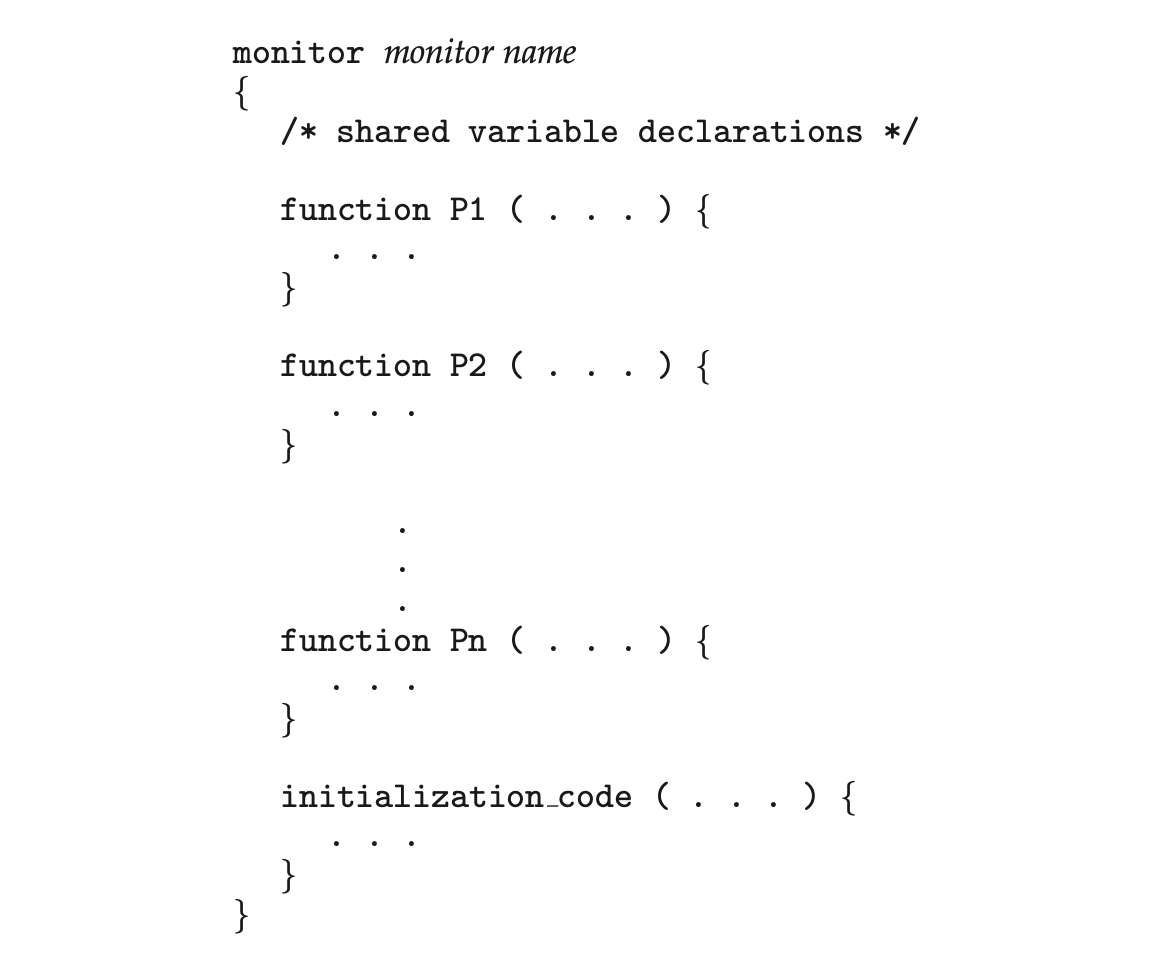
\includegraphics[width=\textwidth]{Pictures/monitorPseudocode.png}
	\caption{Struttura di un monitor in pseudocodice.}
\end{figure}
Le variabili dichiarate in un monitor formano lo \textbf{stato} del monitor e le funzioni definite nel monitor possono accedere solamente alle variabili dello stato, oltre che a quelle dichiarate localmente alla funzione ovviamente. Il monitor garantisce inoltre che un solo processo alla volta possa essere attivo all'interno del monitor (mutua esclusione).
Il monitor è provvisto di un ulteriore meccanismo di sincronizzazione dato dal costrutto \emph{condition}. Le uniche operazioni che possono essere invocate su una variabile condition sono \emph{wait()} e \emph{signal()}, le quali si comportano in maniera simile alle operazioni \emph{P()} e \emph{V()} dei semafori. Tuttavia \emph{wait()} blocca \textbf{sempre} il processo che la chiama e \emph{signal()} svaglia esattamente un solo processo, se non c'è nessun processo in attesa non succede nulla. Nel caso di \emph{signal} ci sono due comportamenti possibili:
\begin{itemize}
	\item \textbf{Signal and wait}. Il processo che ha chiamato signal attende e l'esecuzione passa al processo che si è sbloccato.
	\item \textbf{Signal and continue}. Il processo che ha chiamato signal continua la sua esecuzione ed esce dal monitor (in questo caso signal deve essere l'ultima istruzione della procedura).
\end{itemize}

Per concludere la trattazione sui monitor bisogna evidenziare come, sebbene essi siano più semplici da utilizzare per il programmatore, pochi linguaggi li implementano e per funzionare necessitino di memoria condivisa.

\section{Classi syncronized in Java}
Java come linguaggio ad alto livello fornisce un suo meccanismo per la sincronizzazione dei processi ovvero la keyword \emph{\textbf{syncronized}}.
Un metodo \emph{syncronized} è un metodo che può essere eseguito da una sola thread alla volta. Ciò viene realizzato mantendendo un singolo lock (detto monitor, ma da non confondere con i monitor trattati in precedenza) per oggetto. Se il metodo \emph{syncronized} è statico allora il lock viene messo sulla classe.
E' possibile inoltre definire una sezione critica su qualsiasi blocco utilizzando sempre la keyword \emph{syncronized}.
Sono disponibili inoltre altri metodi di sincronizzazione disponibili nella classe Object e quindi ereditati da tutti gli oggetti, ovvero \emph{\textbf{wait()}, \textbf{notify()}, \textbf{notifyAll()}}.
